% 用极值点确定函数图像

\pentry{导数与函数的极值\upref{DerMax}}

许多时候,我们可以通过函数极值点的位置以及种类确定函数的大致图像.

\begin{exam}{}
求以下函数的极值点,并判断该函数的大致图像
\begin{equation}
f(x) = a + \frac{b}{2} x^2 - \frac{c}{4} x^4 + \frac{d}{6} x^6 \quad (a,b,c,d >0)
\end{equation}

\begin{figure}[ht]
\centering
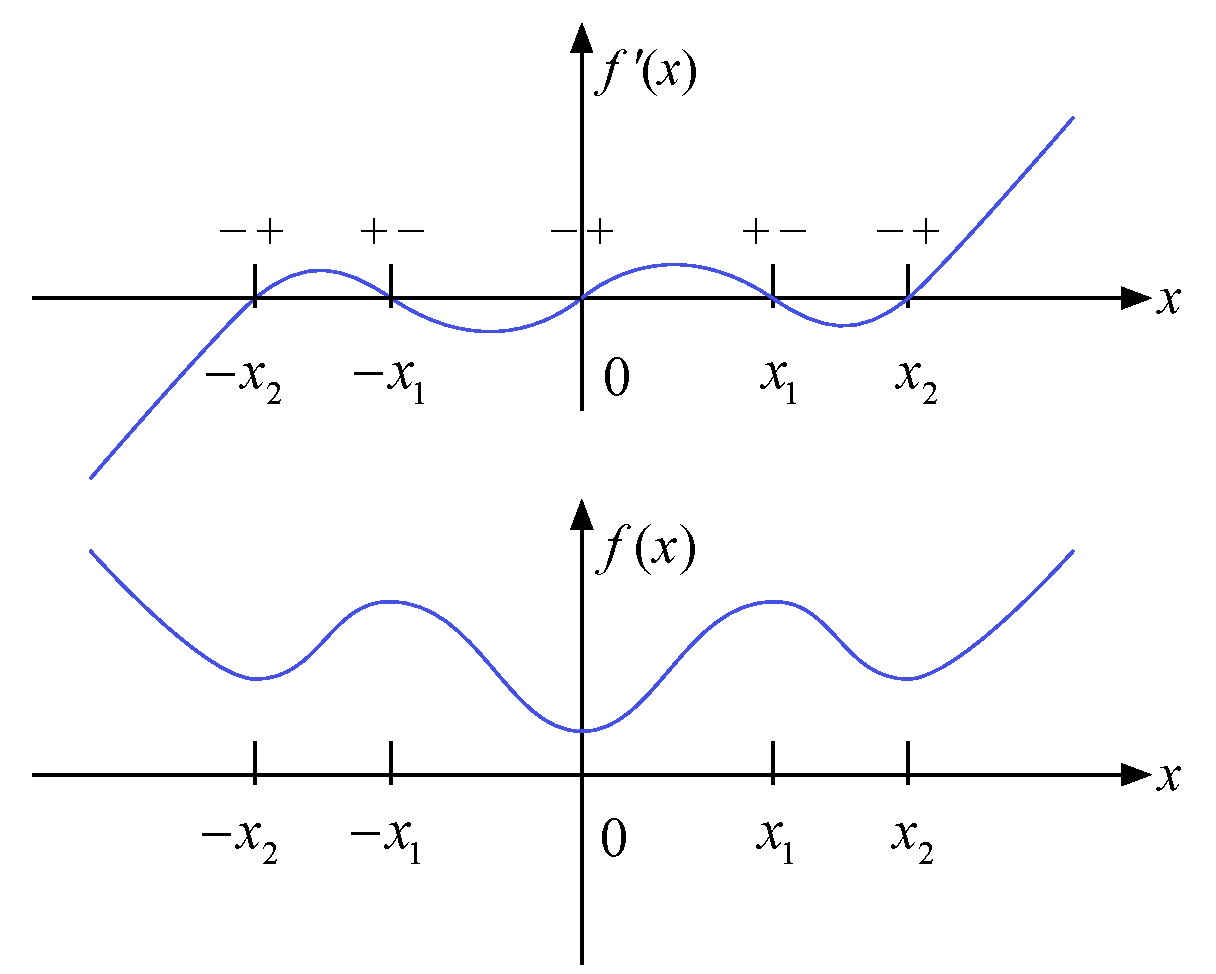
\includegraphics[width=9cm]{./figures/DerImg.pdf}
\caption{导数 $f'(x)$ 与原函数 $f(x)$}\label{DerImg_eq1}
\end{figure}

先对函数求导,得
\begin{equation}
f'(x) = bx - c x^3 + d x^5
\end{equation}
这是一个 $5$ 次多项式,最多可能有五个零点.但由于多项式只有奇数项,不难解出可能的根.
 \begin{equation}
bx + c x^3 + d x^5 = x[b + c(x^2) + d(x^2)^2 ]
\end{equation}
所以其中一个解是 $x = 0$, 而 $b + c(x^2) + d (x^2)^2$ 是关于 $x^2$ 的二次方程,当判别式 $\Delta  = c^2 - 4bd$ 大于零时, $x^2$ 存在两个大小不等的正根,姑且记为 $x_1^2$ 和 $x_1^2$, $x_1 < x_2$. 
此时五个根分别为 $0, \pm x_1, \pm x_2$. 
\begin{equation}
f'(x) = d \cdot x (x^2 - x_2^2) (x^2 - x_2^2) = d \cdot x (x + x_1)(x - x_1)(x + x_1)(x - x_2)
\end{equation} 
由于 $d > 0$, 可以大致画出 $f'(x)$ 图像如\autoref{DerImg_eq1}(下).

用二阶导数判断分类.若二阶导数为正,则是极小值,若为负,则是极大值,若为零,则是鞍点.
\end{exam}
